\chapter{Introduction}
\label{chap:intro}
\chaptoc{}

% ########################################

\newpage
\section{Gravitational Waves}
\label{sec:gw}
\begin{colsection}

% ~~~~~~~~~~~~~~~~~~~~

\begin{colsection}

Einstein's theory of General Relativity describes gravity as the curvature of spacetime \citep{Einstein1914}, and he went on to describe the propagation of distortions within the spacetime `fabric' \citep{Einstein1916}. These \emph{gravitational waves} (GWs) \glsadd{gw} are produced by the acceleration of matter within the field of spacetime and propagate at the speed of light, analogous to electromagnetic (EM) \glsadd{em} waves being produced by a moving charge. The existence of gravitational waves is a consequence of the finite propagation time of gravity in general relativity, there is no analogue to gravitational waves in Newtonian gravity as Newton described a force propagating instantaneously.

The result of Einstein's quadrupole equations is the theory that gravity propagates as a transverse wave, which alternately stretches and compresses spacetime in two orthogonal axes \citep{BIGcardiff}. A single object will never `observe' a gravitational wave, as it is embedded in the fabric, and the only way to detect the passing of gravitational waves is to look for changes in the relative positions of two or more objects as the wave passes through. A thought experiment considering the effects of gravitational waves on free-floating masses is shown in \aref{fig:wave}, for the two wave polarisation states. The magnitude of these perturbations is described as the strain, and it is the goal of gravitational wave detectors to observe these minute spatial perturbations as the wave passes through.

A detailed discussion of general relativity and gravitational wave science is beyond the scope of this thesis, so this section gives merely a brief introduction to the topic in order to explain the core purpose of the GOTO project.

\begin{figure}[t]
    \begin{center}
        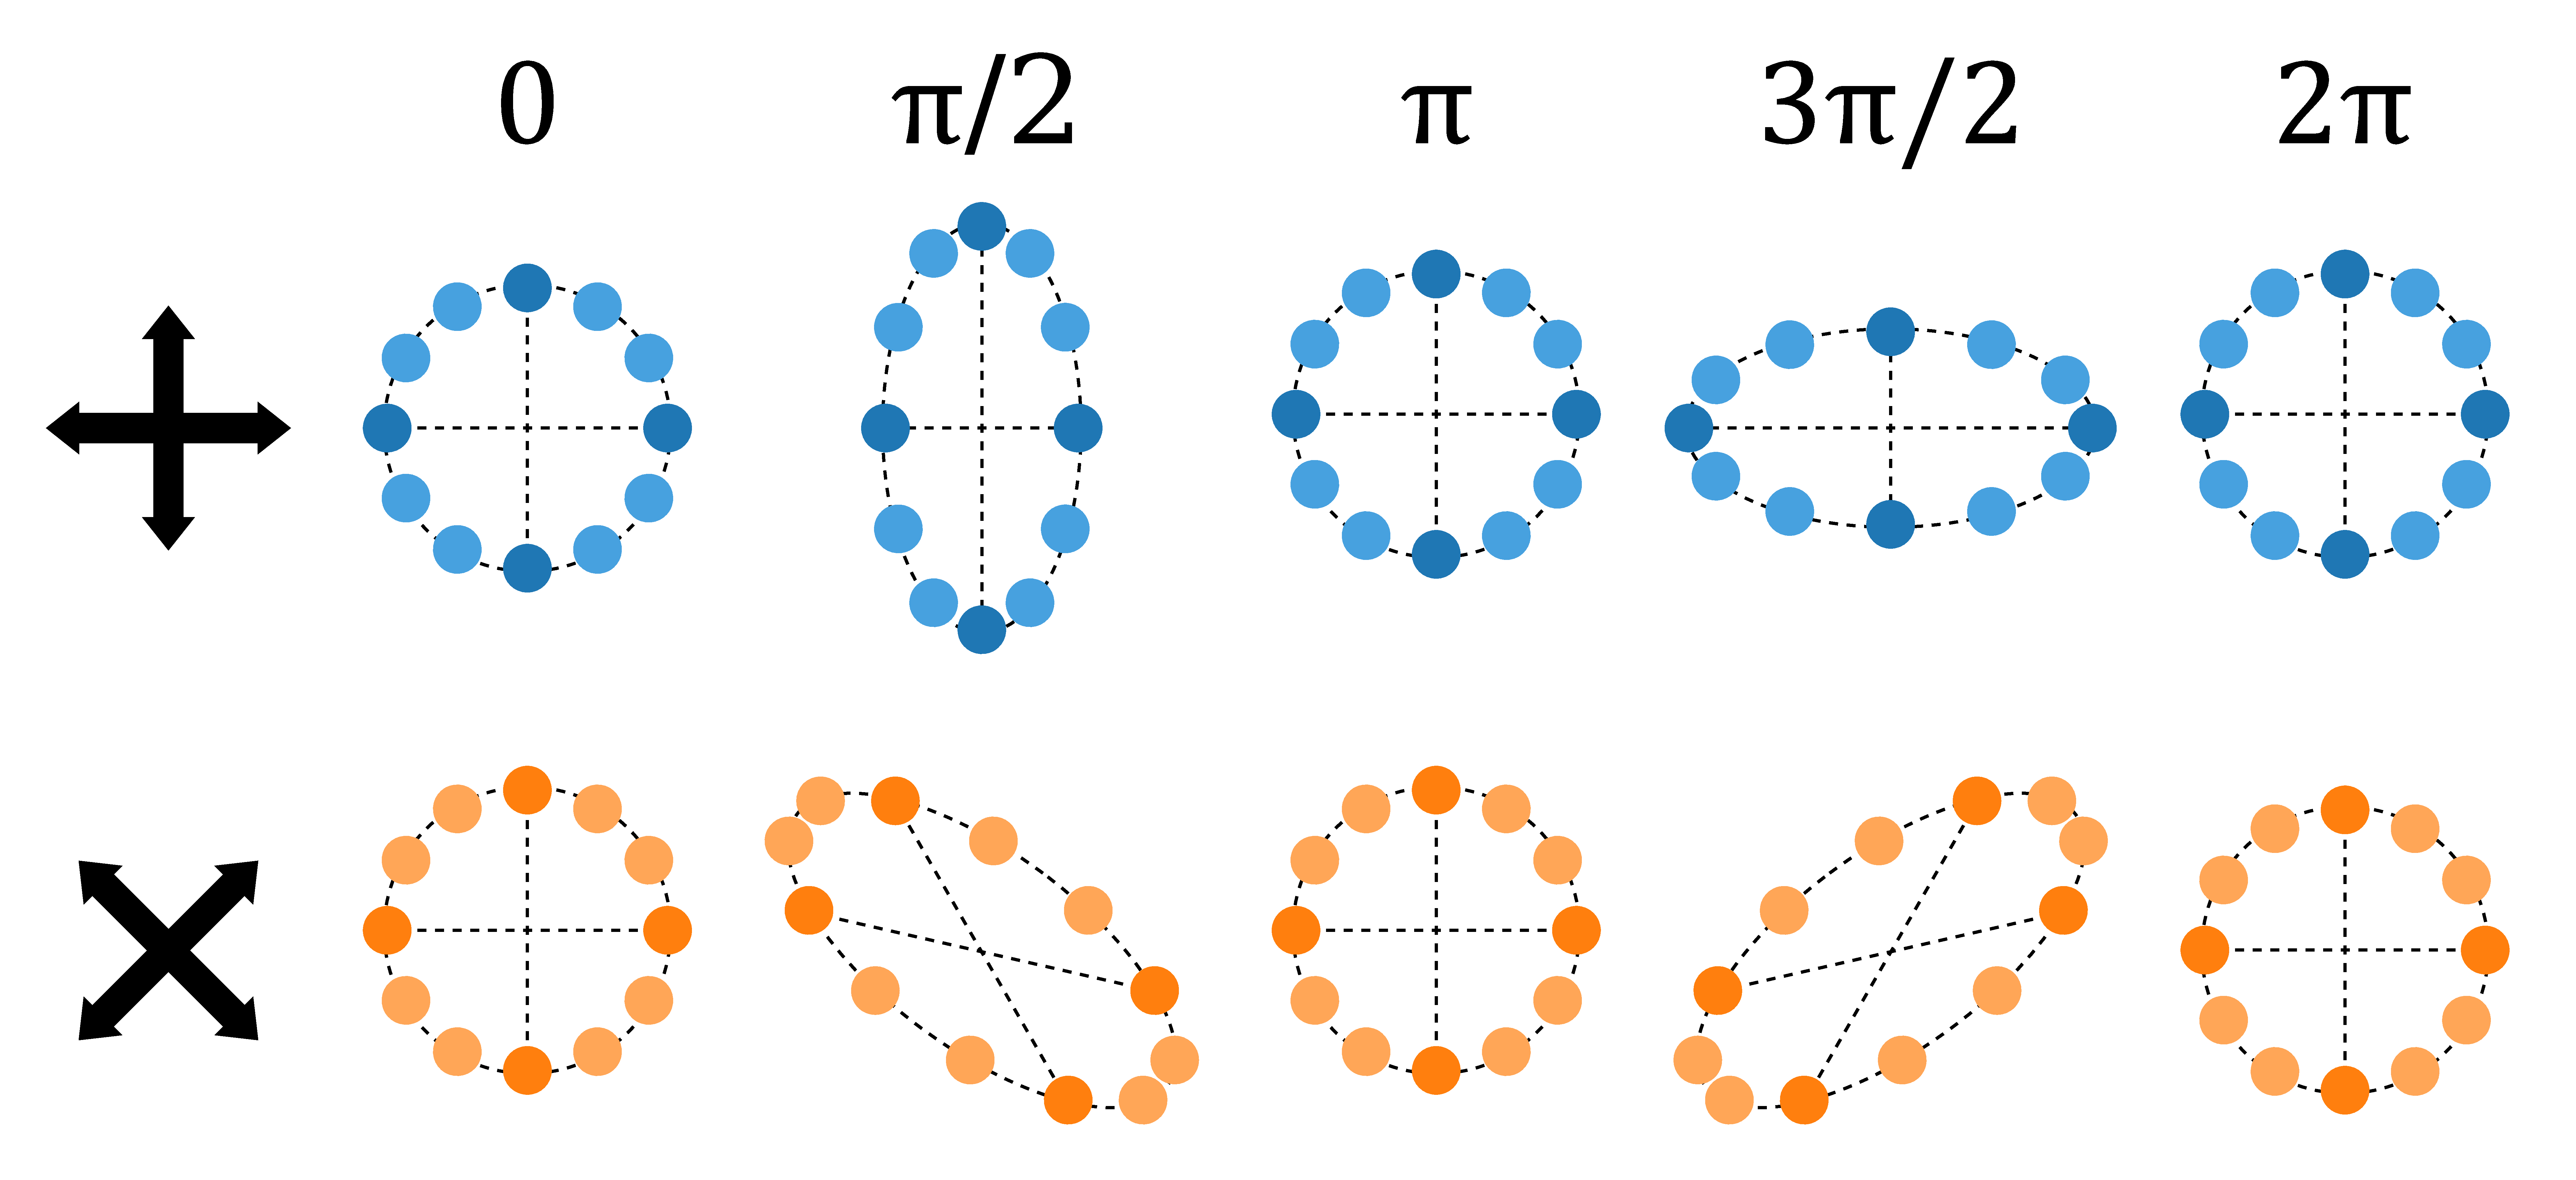
\includegraphics[width=0.8\linewidth]{images/waveimg2.pdf}
    \end{center}
    \caption[Gravitational wave polarisations]{
        Consider a 2-dimensional ring of free-floating particles in the $x$-$y$-plane. A gravitational wave which passes through the ring in the $z$-direction (out of the page) will alternately stretch and compress the ring in two orthogonal axes out of phase. The upper image shows the effect of a plus-polarised wave, the lower image shows the effect of a cross-polarised wave.
        }\label{fig:wave}
\end{figure}

\end{colsection}

% ~~~~~~~~~~~~~~~~~~~~
\newpage
\subsection{Detecting gravitational waves}
\label{sec:gw_detecting}
\begin{colsection}

As described above, gravitational waves manifest as alternately stretching and compressing spacetime along perpendicular axes. Several methods of directly detecting gravitational waves has been proposed, but the most successful design uses a Michelson interferometer to observe how two test masses move relative to each other as a wave passes through. \citep{BIGbirmingham}. As shown in \aref{fig:detector}, the input laser is split into two by a beam spitter and each beam is sent into one of the two long perpendicular arms. Each arm acts as a laser cavity, reflecting the beam multiple times between two mirrored test masses. When they exit the arms the beams are recombined to form a single output. Should the lengths of the arms change relative to each other the distance the beams travel will be different, which will produce a chance in the resulting interference pattern produced when they recombine. The test masses are suspended by a complex vibration isolation system in order to reduce any outside interference, such as from man-made vibrations or seismic events.

\begin{figure}[p]
    \begin{center}
        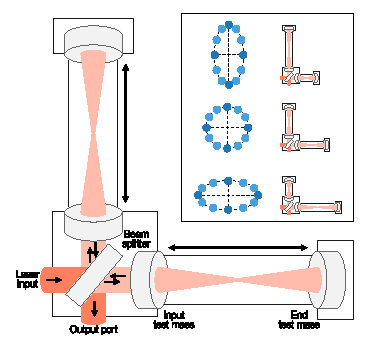
\includegraphics[width=0.75\linewidth]{images/detector.pdf}
    \end{center}
    \caption[A Michelson interferometer used as a gravitational wave detector]{
        A Michelson interferometer used as a gravitational wave detector. As a wave passes through the relative lengths of the arms will change, as shown (highly exaggerated) in the inset. This will reduce or increase the distance the laser light travels through each arm and therefore alter the output interference signal. Adapted from \citet{GW150914_detectors}.
        }\label{fig:detector}
\end{figure}

\begin{figure}[p]
    \begin{center}
        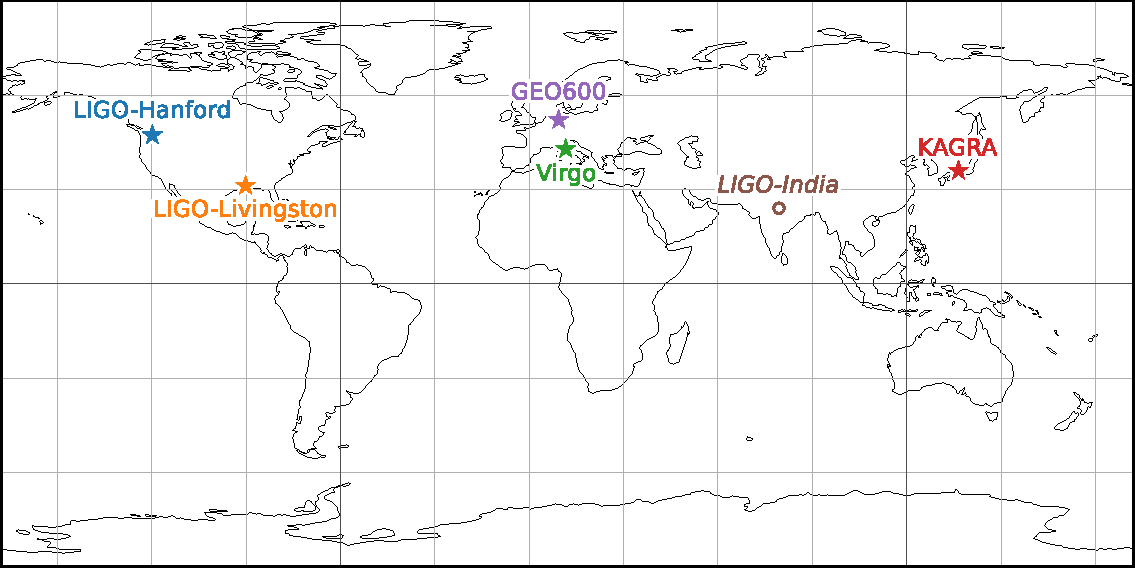
\includegraphics[width=0.95\linewidth]{images/global.pdf}
    \end{center}
    \caption[Locations of gravitational wave detectors]{
        Locations of current and proposed gravitational wave detectors.
        }\label{fig:global}
\end{figure}

\newpage

Several of these gravitational wave detectors have been built around the world, as shown in \aref{fig:global}. Having multiple detectors acting together provides redundancy, and allows the source of the signal to be localised (see \aref{sec:gw_localisation}). There are currently three active second-generation detectors: the two \glsfirst{ligo} detectors in the United States, at Hanford, Washington and Livingston, Louisiana \citep{LIGO}, and the \glsfirst{ego} Virgo detector near Pisa, Italy \citep{Virgo}. Theses three detectors form a global network as the LIGO-Virgo Collaboration \glsadd{lvc} \citep[LVC,][]{LIGO-Virgo}. In addition the older GEO600 detector in Germany is still in use, primarily as a technology test system \citep{GEO600}. In Japan the \glsfirst{kagra} is currently under construction \citep{KAGRA}, and is expected to join the global network before the end of 2019 \citep{LIGO-Virgo-KAGRA}. In the next decade work should also begin on building a third LIGO detector, LIGO-India \citep{LIGO_India}, relocating an instrument that was previously at Hanford.

In the longer term the third generation of larger and more sensitive gravitational wave telescopes is already being planned, including the Einstein Telescope \citep{EinsteinTelescope} and the Cosmic Explorer \citep{CosmicExplorer}. As well space-based gravitational wave detectors are being planned, such as the Laser Interferometer Space Antenna \glsadd{lisa} \citep[LISA,][]{LISA}. Detectors in space would be free from the seismic noise that limits ground-based detectors at low frequencies, and could therefore detect lower-frequency gravitational waves. This could potentially include signals from supermassive black holes and lower-mass binaries within our own galaxy.

\end{colsection}

% ~~~~~~~~~~~~~~~~~~~~

\subsection{Sources of gravitational waves}
\label{sec:gw_sources}
\begin{colsection}

Any accelerating mass will generate gravitational waves as it moves through spacetime, as long as the motion is not spherically symmetric (e.g.\ a rotating disk or a uniformly expanding sphere) \citep{BIGcardiff,BIGparis}. In practice it is impossible to detect gravitational waves from anything but the most massive objects moving at the fastest speeds, as only they will produce large enough strains.

A continuous source of gravitational waves will be generated by two massive objects orbiting one another \citep{GW_sources}, and the loss of energy from the system in the form of gravitational waves will slowly cause the orbiting distance of the two objects to shrink. The first binary pulsar was discovered in 1974 \citep{HulseTaylor}, and after repeated observations it was apparent that the orbital period of the two stars was decreasing in perfect alignment with the predictions given by general relativity. This was the first real evidence, albeit indirect, of the existence of gravitational waves, and the discovery of the Hulse-Taylor pulsar was deemed so significant that its discoverers were awarded the Nobel Prize in 1993 \citep{HulseTaylor2}.

Due to the loss of energy in the form of gravitational radiation any binary orbit will slowly decay. As the orbital distance decreases so will the period, resulting in the objects orbiting faster and the system emitting gravitational waves at a higher frequencies. This will produce a characteristic `chirp' signal until the two objects eventually collide and produce a huge burst of energy \citep{GW_sources, BIGparis}. The more massive the objects in the system the stronger the signal produced, and so the ideal binary systems for gravitational wave detections are binary neutron stars (BNS) \glsadd{bns}, binary black holes (BBH) \glsadd{bbh} or neutron star-black hole (NSBH) \glsadd{nsbh} binaries.

\end{colsection}

% ~~~~~~~~~~~~~~~~~~~~

\subsection{Gravitational wave detection history}
\label{sec:gw_detections}
\begin{colsection}

The LIGO detectors became operational in 2002 and observed on-and-off until 2010 without detecting any gravitational wave signals, when they were taken offline in order to upgrade into Advanced LIGO \citep{LIGO_initial, LIGO_advanced}.

The detectors were recommissioned in 2015, and first direct detection of gravitational waves occurred on the 14th of September 2015, while the two LIGO detectors were still in engineering mode. The signal, GW150914\footnote{Confirmed gravitational wave detections are named in the form GW\textit{YYMMDD}.}, was produced by the merger of a binary black hole system approximately \SI{440}{\mega\parsec} away with component masses of \SI{35}{\solarmass} and \SI{30}{\solarmass} \citep{GW150914}. The `chirp' signals recorded in the LIGO detectors are shown in \aref{fig:chirp}. Note that the fractional strain on the $y$-axis is of the order of $10^{-21}$, meaning as the wave passed through the \SI{4}{\kilo\metre}-long LIGO detector arms changed in length by a fraction of the size of a proton.

\begin{figure}[t]
    \begin{center}
        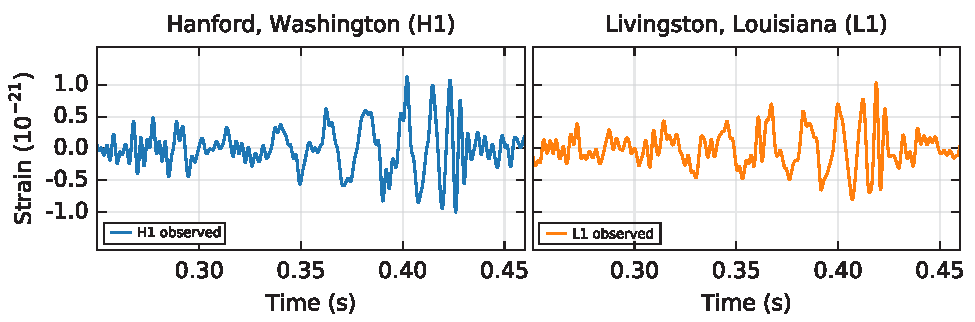
\includegraphics[width=\linewidth]{images/chirp.pdf}
    \end{center}
    \caption[The first detection of gravitational waves]{
        The first detection of gravitational waves, recorded in the LIGO Hanford detector (left) and then approximately \SI{7}{\milli\second} later in the LIGO Livingston detector (right). Adapted from \citet{GW150914}.
        }\label{fig:chirp}
\end{figure}

The first LIGO observing run (O1) \glsadd{o1} continued from September 2015 to January 2016, and during that time two additional signals were detected \citep{LIGO_O1}. All three detections were identified as being produced by coalescing black hole binaries, and although at the time one (LVT151012) was below the $5\sigma$ significance level it has since been upgraded to a significant detection and reclassified as GW151012 \citep{GW_catalog}.

The second observing run (O2) \glsadd{o2} took place from November 2016 to August 2017. This run saw the first observation of gravitational waves from a binary neutron star, GW170817 \citep{GW170817}, as well as the addition of the Virgo detector to the network. In total eleven gravitational wave events were detected during O1 and O2, ten from binary black holes and just the one (GW170817) from a binary neutron star \citep{GW_catalog}.

After a few short engineering runs the third observing run (O3) \glsadd{o3} begun on 1 April 2019. At the time of writing it is currently ongoing, and after a short break during October is expected to run until May 2020. This is the first run to include the three LIGO-Virgo detectors from the beginning, and KAGRA is also expected to join before the end of 2019. This run also marked the start of public alert releases; during O1 and O2 alerts were only released to groups who had signed memoranda of understanding with the LVC (the GOTO Collaboration was one of these groups). In the first 5 months of O3, from the start of April to the end of August 2019, the LVC released 32 alerts\footnote{Public alerts are available at \url{https://gracedb.ligo.org/superevents/public/O3/}}. Of these 7 were ultimately retracted as false alarms, leaving 25 due to real astronomical signals.

As O3 is currently ongoing the LVC has not yet published final values or mass estimates for any of these events. As such they are still treated as candidates, with provisional signal designations and preliminary classification probabilities. Of the 25 non-retracted events 20 are currently classified as originating from binary black hole systems ($P_\text{BBH}>90\%$). Only one is likely from a binary neutron star (S190425z), one is classed as a likely neutron star-black hole binary (S190814bv), and one (S190426c) has an uncertain classification: a 49\% probability as coming from a binary neutron star, 24\% coming from a `MassGap' object (a theorised object with a mass between a neutron star and a black hole) and 13\% from a neutron star-black hole binary (the remaining 14\% is the chance the signal is from a non-astrophysical source, i.e.\ detector noise). The remaining two events both have over 50\% non-astrophysical probability but have not been formally retracted by the LVC.\@

\end{colsection}

% ~~~~~~~~~~~~~~~~~~~~
\newpage
\subsection{On-sky localisation}
\label{sec:gw_localisation}
\begin{colsection}

One problem with the interferometer detectors is that alone they are very poor at localising the direction a signal originates from. It is possible to estimate a rough direction from polarisation of the signal, and the distance to the origin can be estimated from the signal strength, however multiple detectors are really needed to get more accurate sky localisations \citep{GW_localisation, GW_localisation2}. With two detectors the difference between the arrival time of a signal at each allows the direction to the source to be narrowed down, based on the distance between the two detectors and knowing that gravitational waves propagate at the speed of light. However this will only be able to locate the source to a annulus on the celestial sphere perpendicular to the line between the detectors, and as shown in \aref{fig:triangulate} at least three detectors are needed to triangulate the source location. The skymaps for GW170817, shown in \aref{fig:170817_skymaps}, show how the contribution from multiple detectors drastically reduced the on-sky area. Even with the three current detectors sources can typically only be localised to areas of tens to hundreds of square degrees at best, and only if the signal is detected in all three.

\begin{figure}[t]
    \begin{center}
        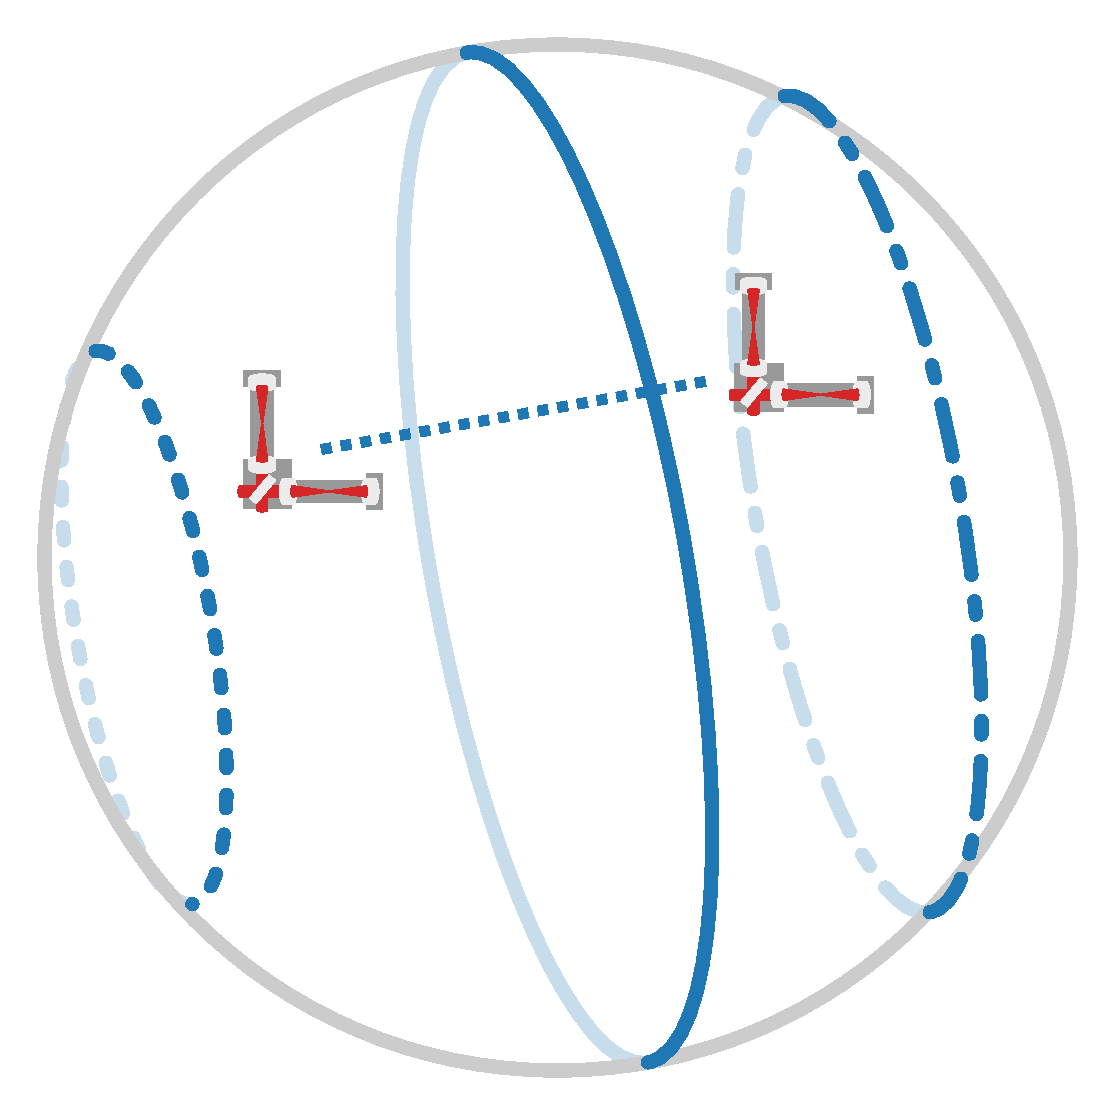
\includegraphics[width=0.4\linewidth]{images/triangulate_1.pdf}
        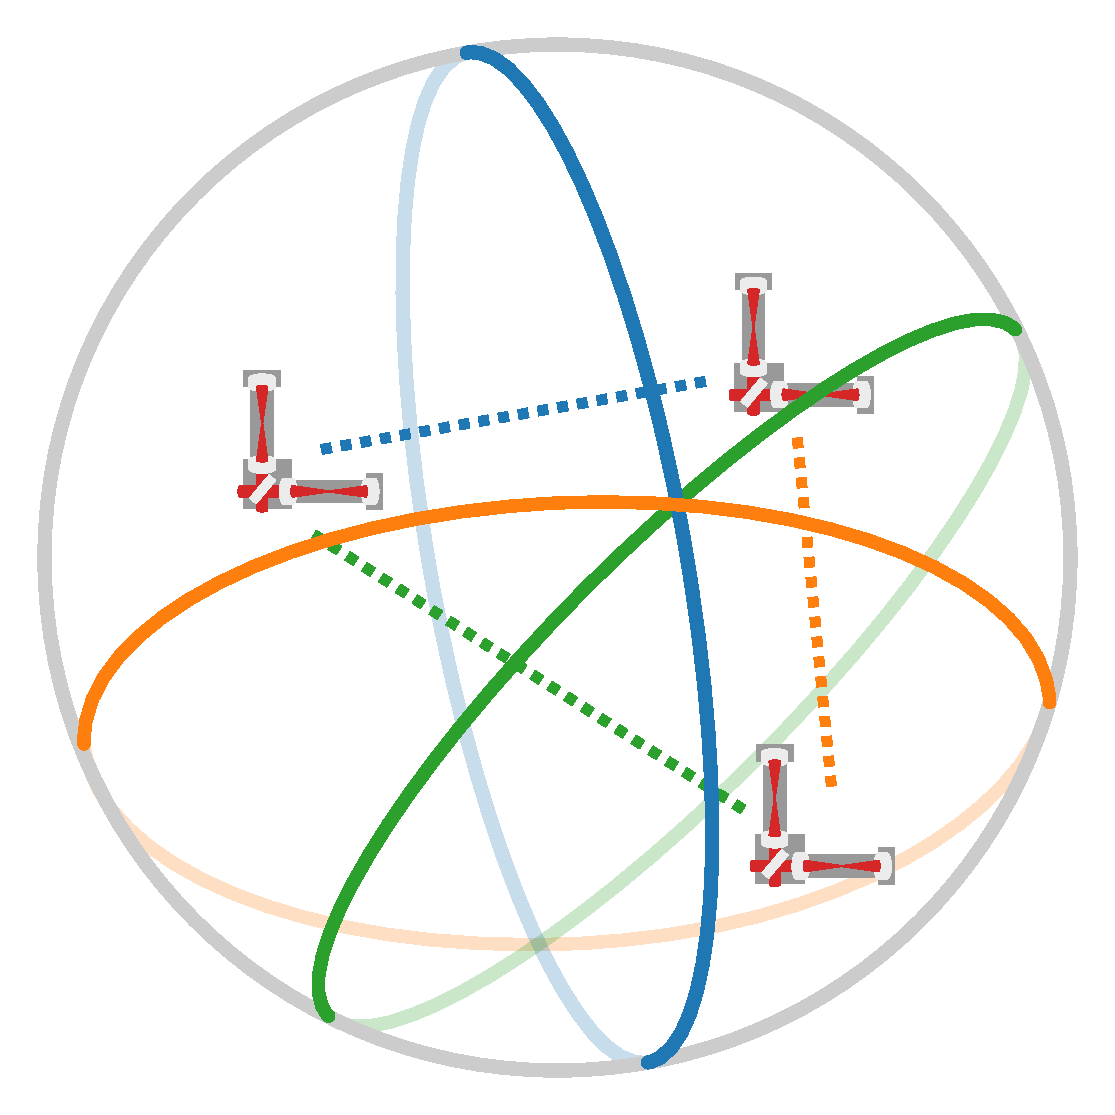
\includegraphics[width=0.4\linewidth]{images/triangulate_2.pdf}
    \end{center}
    \caption[Localising signals using gravitational wave detectors]{
        Localising signals using gravitational wave detectors. With just two detectors sources can only be localised to a ring on the sky (shown on the left, for three different sources). The addition of a third detector means sources can be triangulated to where the rings intercept (shown on the right).
        }\label{fig:triangulate}
\end{figure}

\begin{figure}[p]
    \begin{center}
        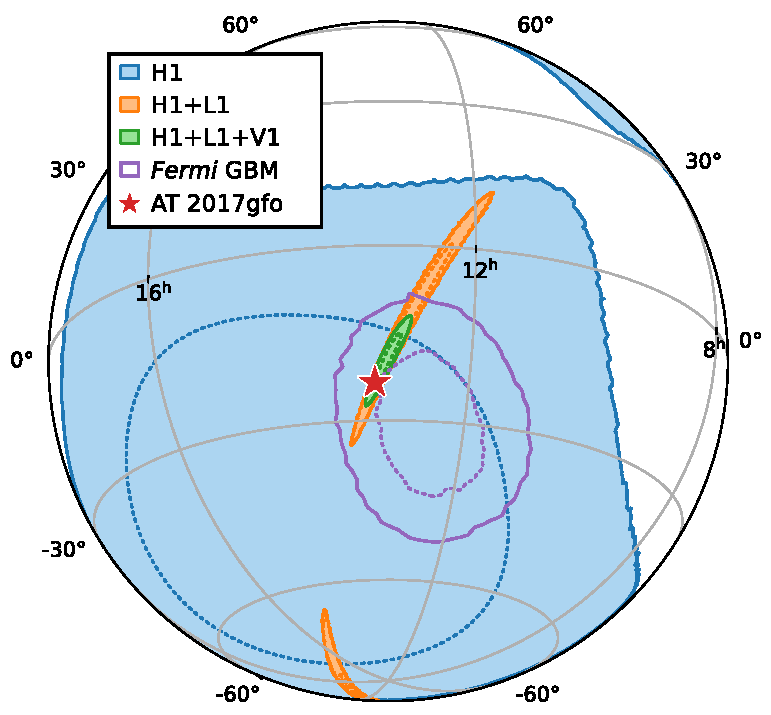
\includegraphics[width=\linewidth]{images/skymaps.pdf}
    \end{center}
    \caption[Skymaps for GW170817]{
        Skymaps for GW170817, produced from the single Hanford detector (in \textcolorbf{NavyBlue}{blue}), both Hanford and Livingston (\textcolorbf{Orange}{orange}) and all three detectors (\textcolorbf{Green}{green}). The final \textit{Fermi} GBM skymap is also shown in \textcolorbf{Purple}{purple}, and the location of the counterpart source is marked by a \textcolorbf{Red}{red} star. Solid lines show 50\% confidence regions, dashed lines 90\% regions.
        }\label{fig:170817_skymaps}
\end{figure}

\end{colsection}

% ~~~~~~~~~~~~~~~~~~~~

\end{colsection}

% ########################################

\newpage
\section{Multi-Messenger Astronomy}
\label{sec:multi}
\begin{colsection}

% ~~~~~~~~~~~~~~~~~~~~

\begin{colsection}

\emph{Multi-messenger astronomy} refers to detecting multiple signals from the same source using two or more different `messengers'. Such messengers can include electromagnetic waves/photons, gravitational waves, neutrinos or cosmic rays. An example of a multi-messenger event would be supernova SN 1987A, which was detected by neutrino detectors several hours before becoming visible in the electromagnetic spectrum \citep{SN1987A}. This thesis concentrates on the search for electromagnetic counterparts to gravitational wave detections, of which at the time of writing only one has been found \citep[GW170817;][]{GW170817}.

Even before GW170817 was detected it had long been theorised that some gravitational wave detections might have electromagnetic counterparts. Binary mergers involving neutrons stars (either neutron star binaries or neutron star-black hole mergers) were suggested as possible source of short duration gamma ray bursts \citep{SGRBs}, and they were expected to produce visible kilonovae \citep{BNSNSBH_EM, BNS_EM}. Electromagnetic counterparts to binary black hole mergers were less expected; binary stellar-mass black holes may not be surrounded by much orbiting matter with which to interact, however certain systems with an orbiting disk might produce enough material for accretion and subsequent emission \citep{BBH_EM}.

\end{colsection}

% ~~~~~~~~~~~~~~~~~~~~

\subsection{The benefits of multi-messenger observations}
\label{sec:mma_benefits}
\begin{colsection}

As explained in \aref{sec:gw_localisation}, gravitational wave detectors have only a limited ability to localise the source location. Wide-field electromagnetic monitors, such as the \textit{Fermi} \glsfirst{gbm}, could provide independent localisation skymaps to help reduce the search area \citep[note the \textit{Fermi} skymap included in \aref{fig:170817_skymaps}]{GW170817_GRB}. Ideally the direct detection of a visible kilonova would allow precise localisation to a host galaxy, as well as a measure of redshift and therefore the distance to the source.

Electromagnetic observations of the counterpart source can give additional insights into the nature of the source objects and their environment, as well as further scientific breakthroughs. For example, observations of the kilonova associated with GW170817 \citep{GW170817, GW170817_followup} allowed analysis of the equation of state of neutron star material \citep{GW170817_NSscience}, an insight into the origin of heavy metals in the universe \citep{GW170818_heavy}, constraints on the nature of gravity \citep{GW170817_gravity} and a new, independent measurement of the Hubble constant \citep{GW170817_hubble}.

At the time of writing GW170817 remains the only confirmed counterpart to a gravitational wave signal. As observations continue and new detectors come online it is only a matter of time until similar objects are found, which will assuredly lead to further astrophysical and cosmological breakthroughs. However future counterparts may not be as easy to find.

\end{colsection}

% ~~~~~~~~~~~~~~~~~~~~

\subsection{Finding optical counterparts to GW detections}
\label{sec:followup}
\begin{colsection}

GW170817 was a remarkably lucky event in several ways. The gravitational wave signal was observed by both LIGO detectors, and although it was not observed by Virgo it was active at the time so the non-detection still helped narrow-down the localisation area. This produced a fairly small skymap, covering just $31~\text{deg}^2$ \citep[see \aref{fig:170817_skymaps}]{GW170817}, which was well positioned for telescopes in the southern hemisphere to observe (although close to the sun the area was visible for a few hours after sunset). The gravitational wave detection also produced a very low luminosity distance of $40\pm\SI{8}{\mega\parsec}$, which made a direct observation feasible. \SI{40}{\mega\parsec} is also close enough to be within the high-completeness range of galaxy catalogues, which helped the search effort.

The first of many observations of the counterpart transient AT 2017gfo was taken by the One-Meter, Two-Hemisphere collaboration using the Swope telescope at Las Campanas Observatory in Chile. The discovery image is shown in \aref{fig:sss17a}, and the Swope team designated the transient SSS17a \citep{GW170817_Swope}. The Swope telescope only has a field of view of $\SI{30}{\arcmin}\times\SI{30}{\arcmin}$, but due to the small, near-by search area a fairly short list of potential host galaxies could be constructed based on the \glsfirst{gwgc} from \citet{GWGC}. The Swope observations could then be targeted to fields including these galaxies, as shown in \aref{fig:swope_decam}. The host galaxy, NGC 4993, was observed in the ninth pointing, and as shown in \aref{fig:sss17a} the kilonova was clearly visible on the outer edge of the galaxy.

\begin{figure}[t]
    \begin{center}
        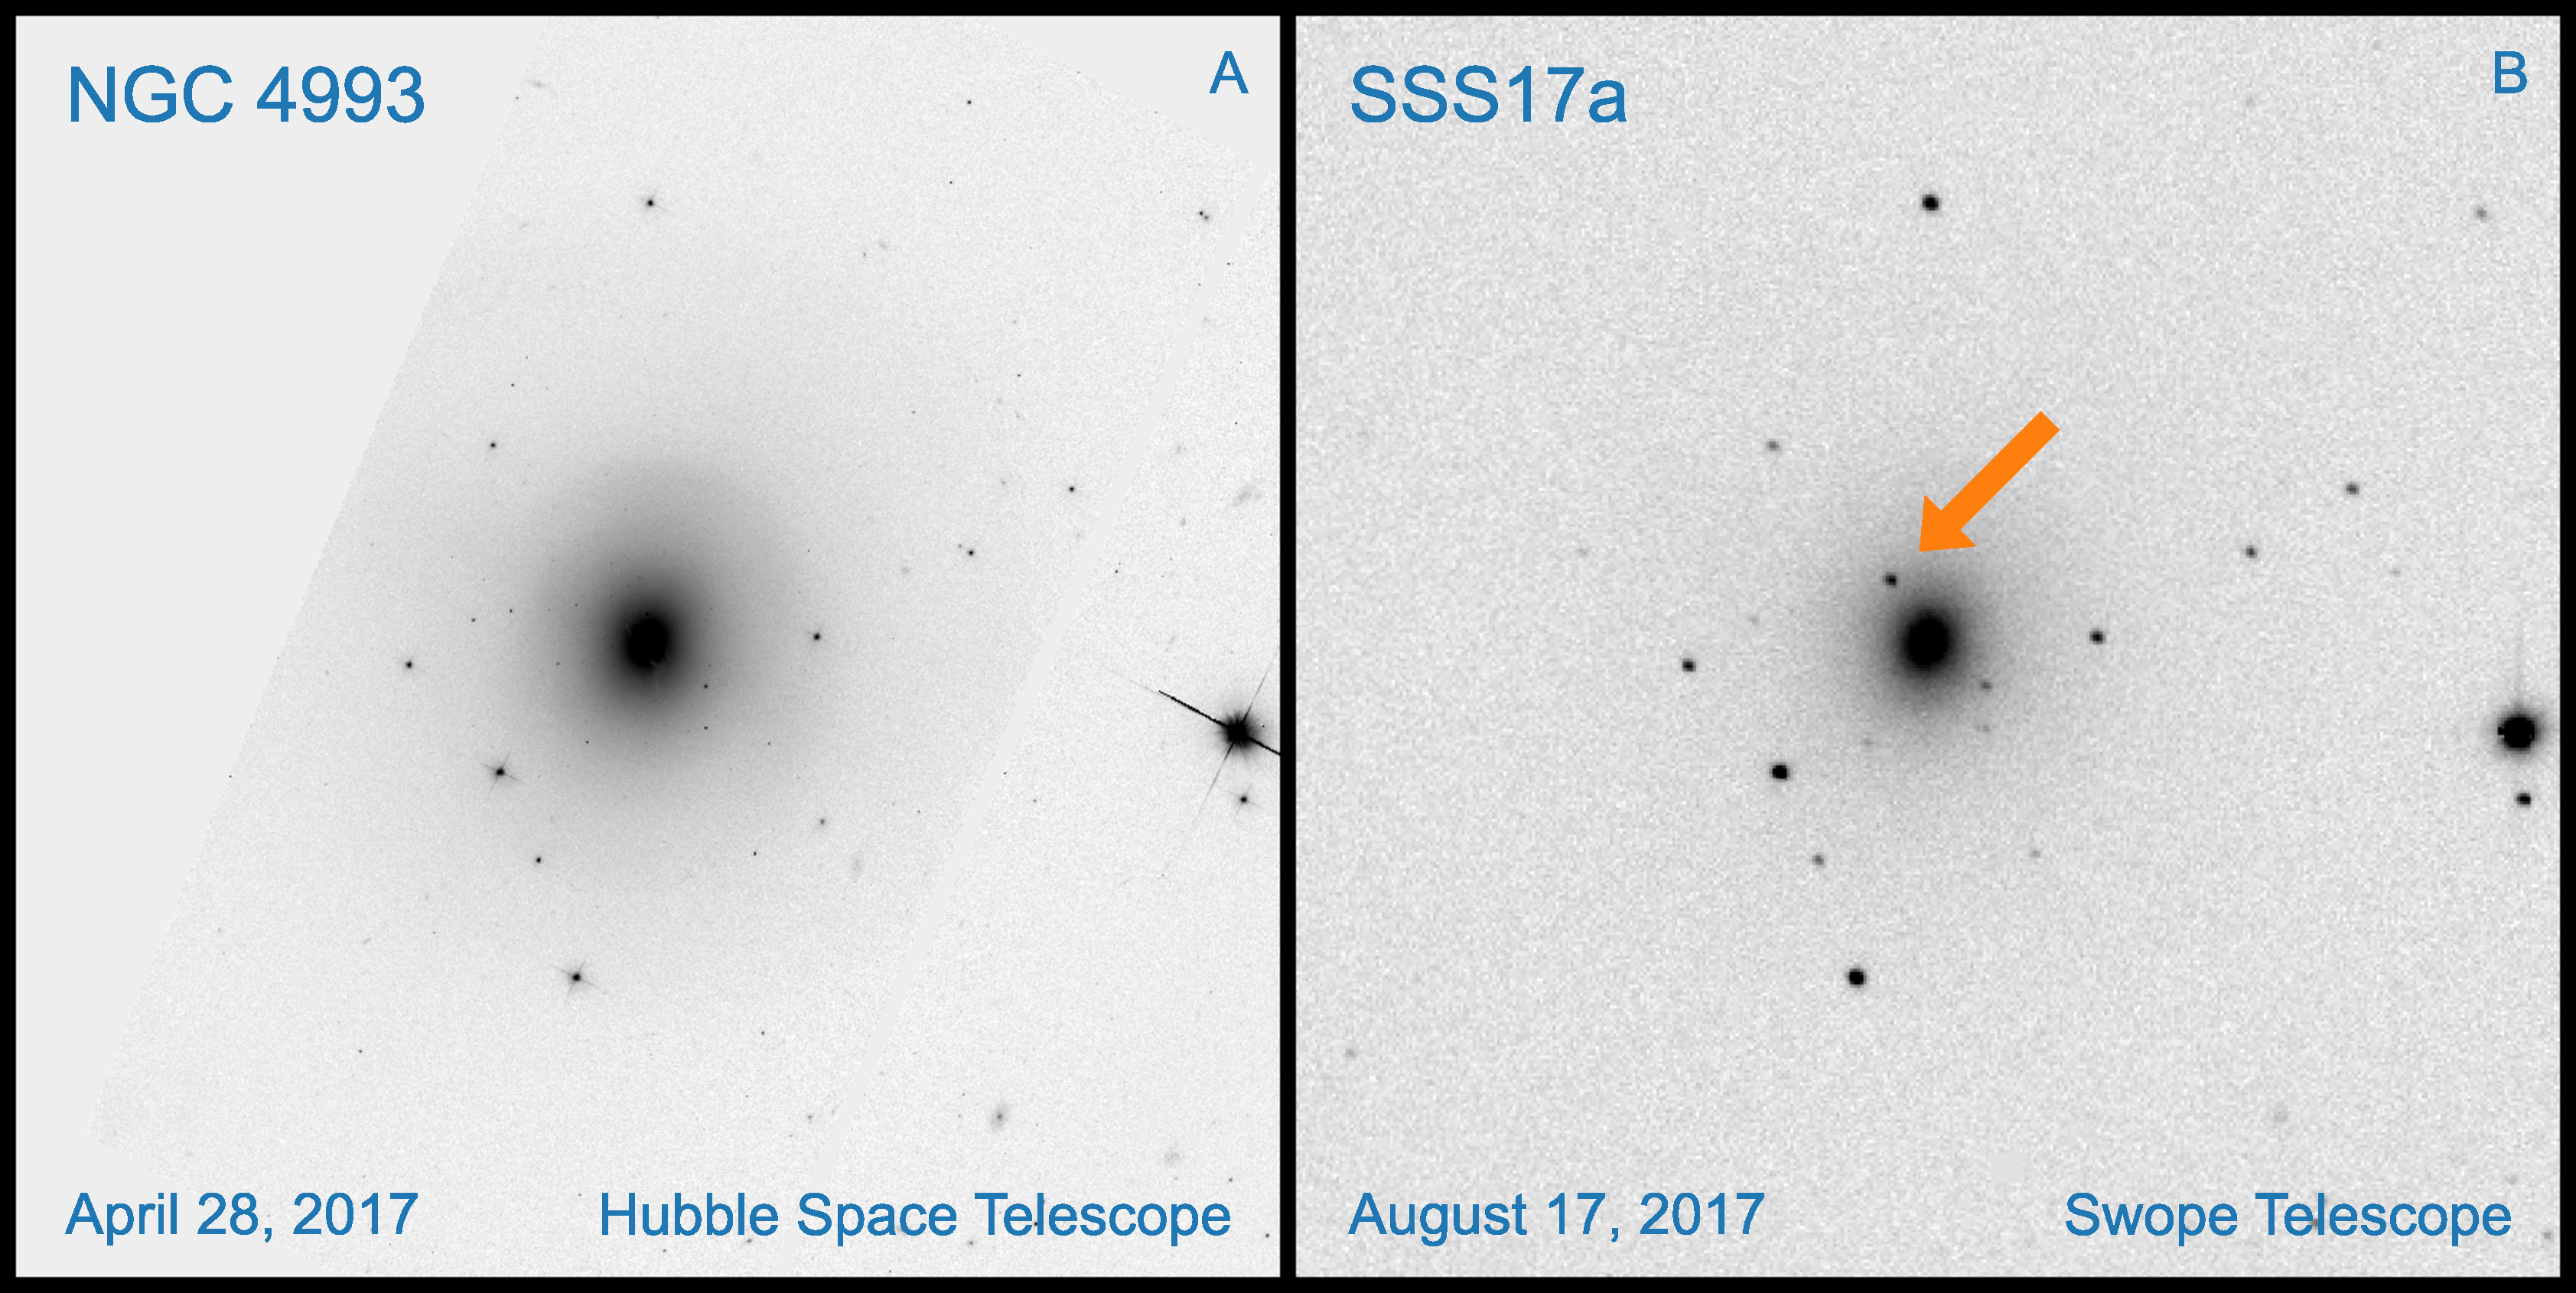
\includegraphics[width=\linewidth]{images/sss17a.pdf}
    \end{center}
    \caption[Detection of the counterpart to GW170817]{
        Detection of the counterpart to GW170817 with the Swope telescope. On the left is an archival image of NGC 4993, and on the right the position of the kilonova is marked. Adapted from \citet{GW170817_Swope}.
        }\label{fig:sss17a}
\end{figure}

\begin{figure}[p]
    \begin{center}
        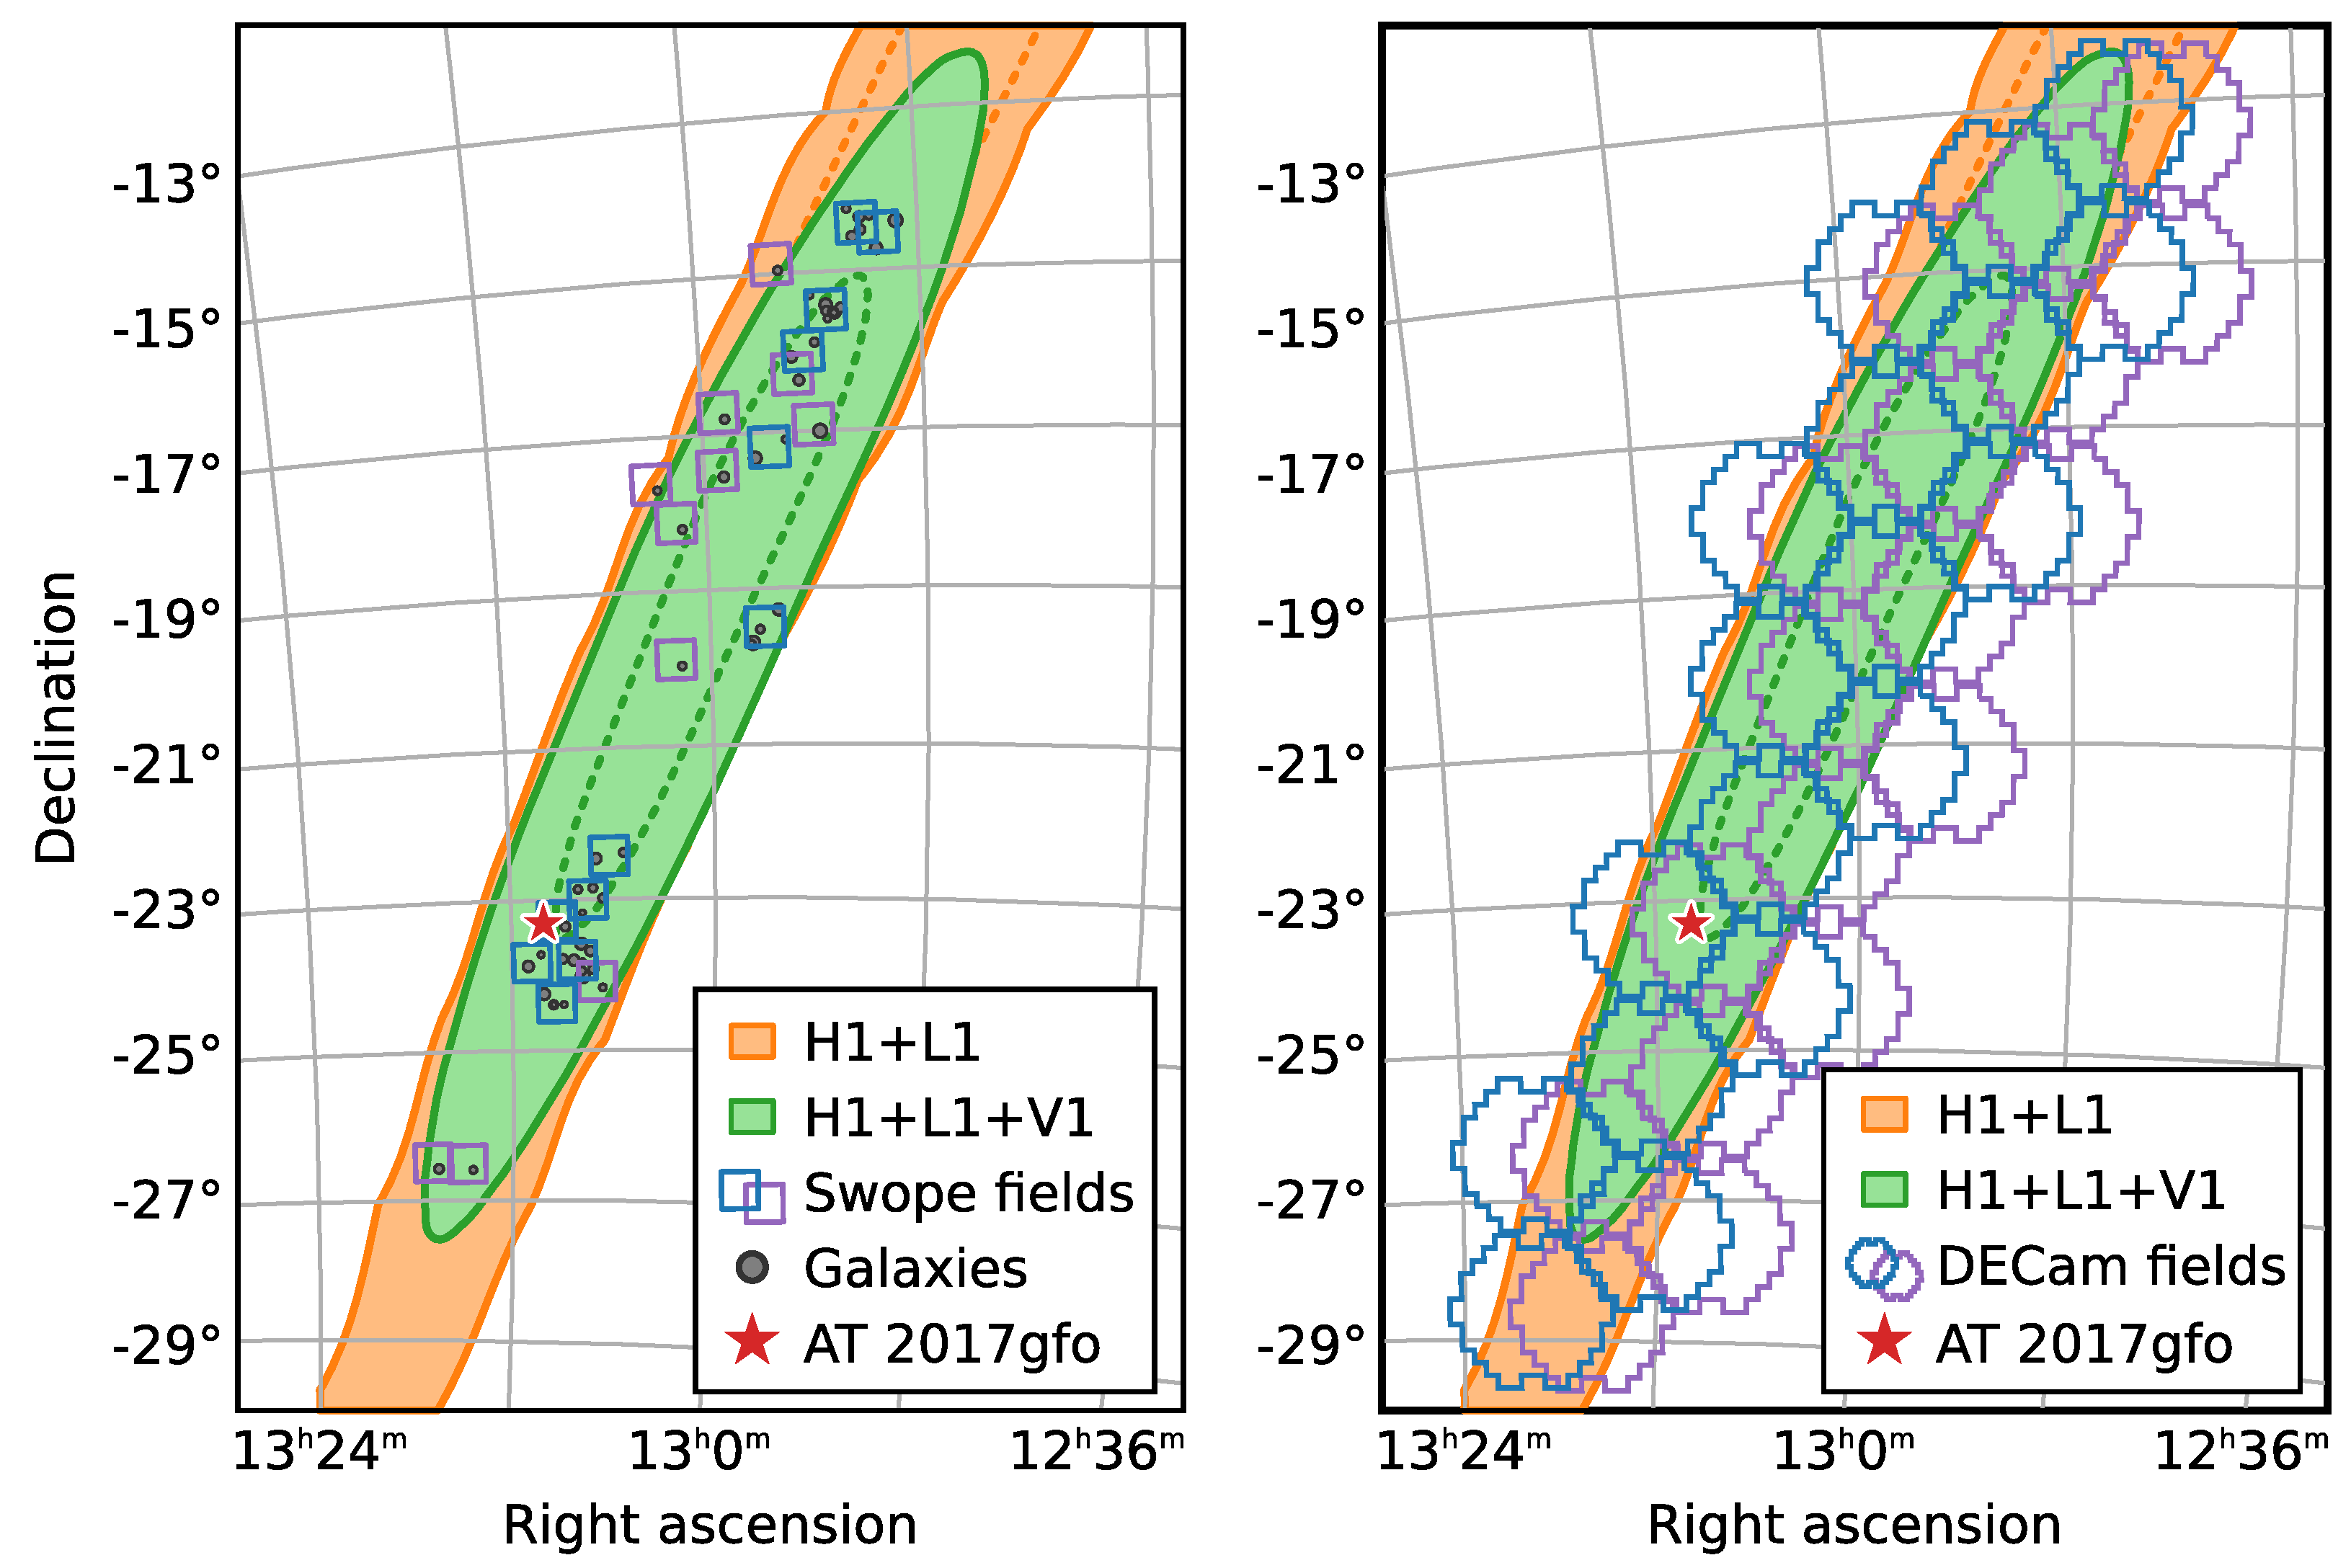
\includegraphics[width=\linewidth]{images/170817_obs.pdf}
    \end{center}
    \caption[Follow-up observations of GW170817 with Swope and DECam]{
        Follow-up observations of GW170817 with the Swope telescope and the Dark Energy Camera. The skymap contours and final transient position are the same as in \aref{fig:170817_skymaps}. \\
        Left: The Swope telescope has a small field of view, and so targeted its follow-up observations on concentrations of GWGC galaxies (\textcolorbf{darkgray}{grey} circles). The \textcolorbf{NavyBlue}{blue} and \textcolorbf{Purple}{purple} squares show the fields observed by Swope containing multiple or single galaxies respectively. Adapted from \citet{GW170817_Swope}.\\
        Right: Instead of targeting galaxies DECam observed using a pre-defined grid of 18 pointings, followed by a second set of offset observations (\textcolorbf{NavyBlue}{blue} and \textcolorbf{Purple}{purple} hexes respectively). Adapted from \citet{GW170817_DECam}.
        }\label{fig:swope_decam}
\end{figure}

Five other groups independently observed the same transient within an hour of the Swope observation: the Dark Energy Camera \glsadd{decam}\citep[DECam,][]{GW170817_DECam}, the Distance Less Than \SI{40}{\mega\parsec} survey \glsadd{dlt40}\citep[DLT40,][]{GW170817_DLT40}, Las Cumbres Observatory \glsadd{lco}\citep[LCO,][]{GW170817_LCO}, the MASTER Global Robotic Net \citep{GW170817_MASTER} and the \glsfirst{eso} Visible and Infrared Survey Telescope for Astronomy \glsadd{vista}\citep[VISTA,][]{GW170817_VISTA}. The observing strategy differed between groups depending on the field of view of the instruments. DLT40 was an existing supernova survey so targeted already-known galaxies, and the LCO and VISTA both targeted their observations to likely host galaxies like Swope. On the other hand DECam and MASTER had larger fields of view, and so could therefore uniformly cover the entire localisation region using a regular `tiling' pattern. The DECam tile pointings are shown on the right plot of \aref{fig:swope_decam}.

The relatively small skymap for GW170817 allowed telescopes with smaller fields of view to efficiently cover the search area, either by targeting galaxies or with a uniform tiling method. However there is no guarantee that this will always be the case, and indeed subsequent events have not been as well localised.

As previously mentioned in \aref{sec:gw_sources} the second binary neutron star gravitational wave detection, S190425z, occurred in April 2019, a few weeks into the O3 run. Unlike GW150914 this was only a single-detector detection, observed only by LIGO-Livingston (again Virgo was also observing at the same time, but LIGO-Hanford was shut down for maintenance). The initial skymap from the BAYESTAR detection pipeline covered an area of approximately 10,000 square degrees, and the final skymap from the LALInference pipeline only reduced this to 7,500~sq~deg; still 250 times the size of the final GW170817 skymap. For searching such large sky areas containing thousands of galaxies the method used by smaller telescopes such as Swope is impractical, and so dedicated wide-field survey telescopes are needed.

The \glsfirst{ztf} is one such telescope, with a field of view of 47~sq~deg. Over the first two nights following the S190425z detection ZTF covered approximately 8,000~sq~deg of the initial skymap \citep{GW190425_ZTF}, shown in \aref{fig:ztf}. This still only corresponded to 21\% of the localisation probability, as unfortunately a large fraction of the skymap was located too close to the Sun to observe.

\newpage

\begin{figure}[t]
    \begin{center}
        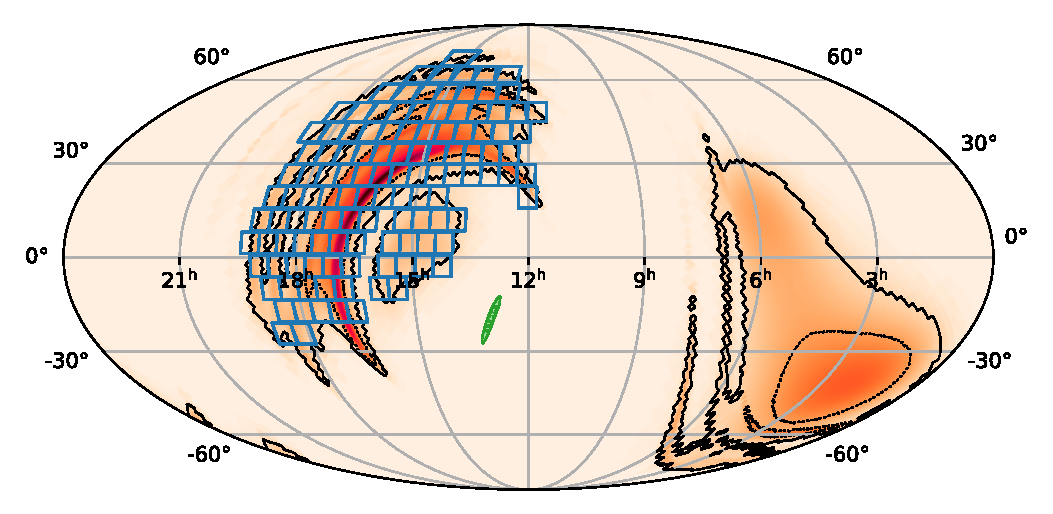
\includegraphics[width=0.9\linewidth]{images/190425_ztf.pdf}
    \end{center}
    \caption[Follow-up observations of S190425z with ZTF]{
        Follow-up observations of S190425z with the Zwicky Transient Facility. The ZTF tiled observations are shown in \textcolorbf{NavyBlue}{blue}, over the background BAYESTAR skymap in \textcolorbf{Orange}{orange}. Adapted from \citet{GW190425_ZTF}. For a size comparison to \aref{fig:swope_decam} the position of the final GW170817 skymap is also shown in \textcolorbf{Green}{green}.
        }\label{fig:ztf}
\end{figure}

If covering the skymap was not enough of a challenge, once observations have been taken a robust analysis pipeline is also needed in order to distinguish potential counterpart candidates from the large number of coincident detections. During the S190425z observations ZTF produced nearly 340,000 transient alerts, which were narrowed down to just 12 potential candidates \citep{GW190425_ZTF}. Ultimately each was shown to be unconnected with the gravitational wave signal, and in the end no likely counterpart was identified for this event by ZTF or any other project.

S190425z was something of an extreme example, and as more gravitational wave detectors come online the typical skymap size should decrease. However it serves as a good counterpoint to the relative ease with which the GW170817 counterpart was found. Small telescopes like Swope can contribute with galaxy-focused observations when the skymap is small enough, but for events like S190425z where large searches are required it is clear that dedicated, wide-field survey telescopes are required to have the best chance of identifying any counterpart.

\end{colsection}

% ~~~~~~~~~~~~~~~~~~~~

\end{colsection}

% ########################################
\clearpage
\newpage
\hfuzz=6pt % It only just overlaps!
\section{The Gravitational-wave Optical Transient Observer}
\hfuzz=.5pt % Reset
\label{sec:goto}
\begin{colsection}

% ~~~~~~~~~~~~~~~~~~~~

\begin{colsection}

The \glsfirst{goto}\footnote{\url{https://goto-observatory.org/}} is a project dedicated to detecting optical counterparts of gravitational wave sources. The GOTO collaboration was founded in 2014 and as of 2019 contains 10 institutions from the UK, Australia, Thailand, Spain and Finland\footnote{The GOTO collaboration includes the University of Warwick, Monash University, Armagh Observatory \& Planetarium, the University of Leicester, the University of Sheffield, the National Astronomical Research Institute of Thailand (NARIT), the Instituto de Astrofisica de Canarias (IAC), the University of Manchester, the University of Turku and the University of Portsmouth.}. The first prototype GOTO telescope was inaugurated at the Roque de los Muchachos Observatory on La Palma, Canary Islands in July 2017 and is shown in \aref{fig:goto_photo}.

\begin{figure}[p]
    \begin{center}
        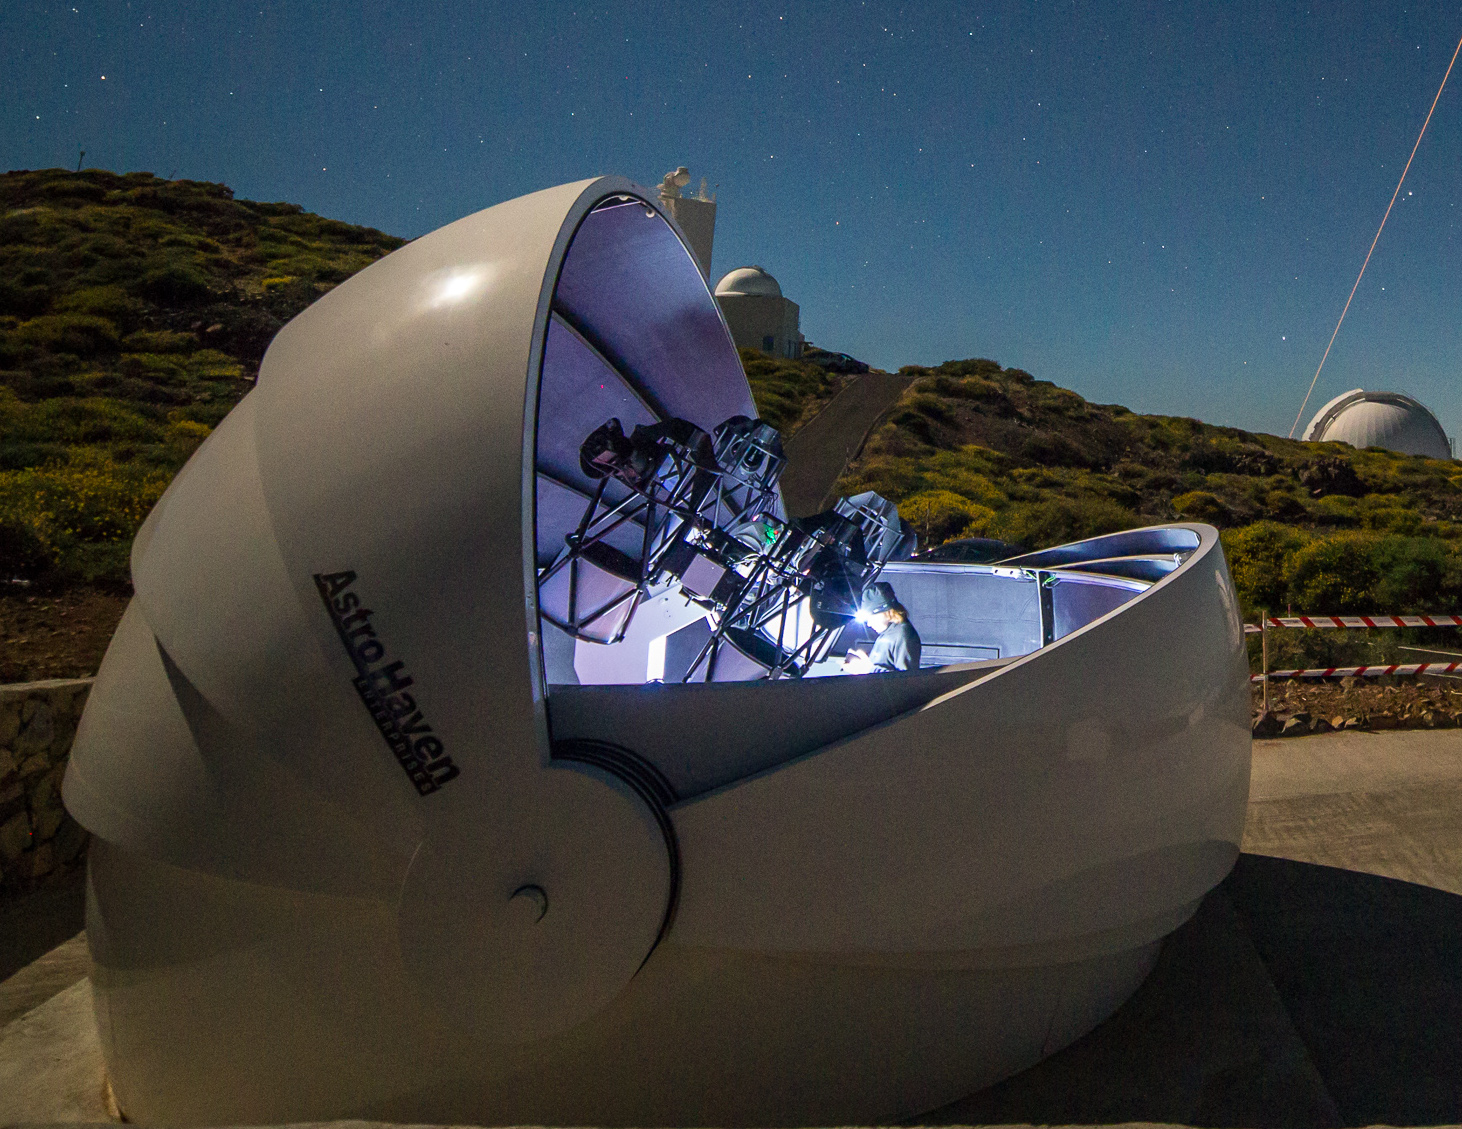
\includegraphics[width=0.9\linewidth]{images/goto_photo.jpg}
    \end{center}
    \caption[The GOTO prototype instrument]{
        The GOTO prototype instrument with four unit telescopes on La Palma.
    }\label{fig:goto_photo}
\end{figure}

\begin{figure}[p]
    \begin{center}
        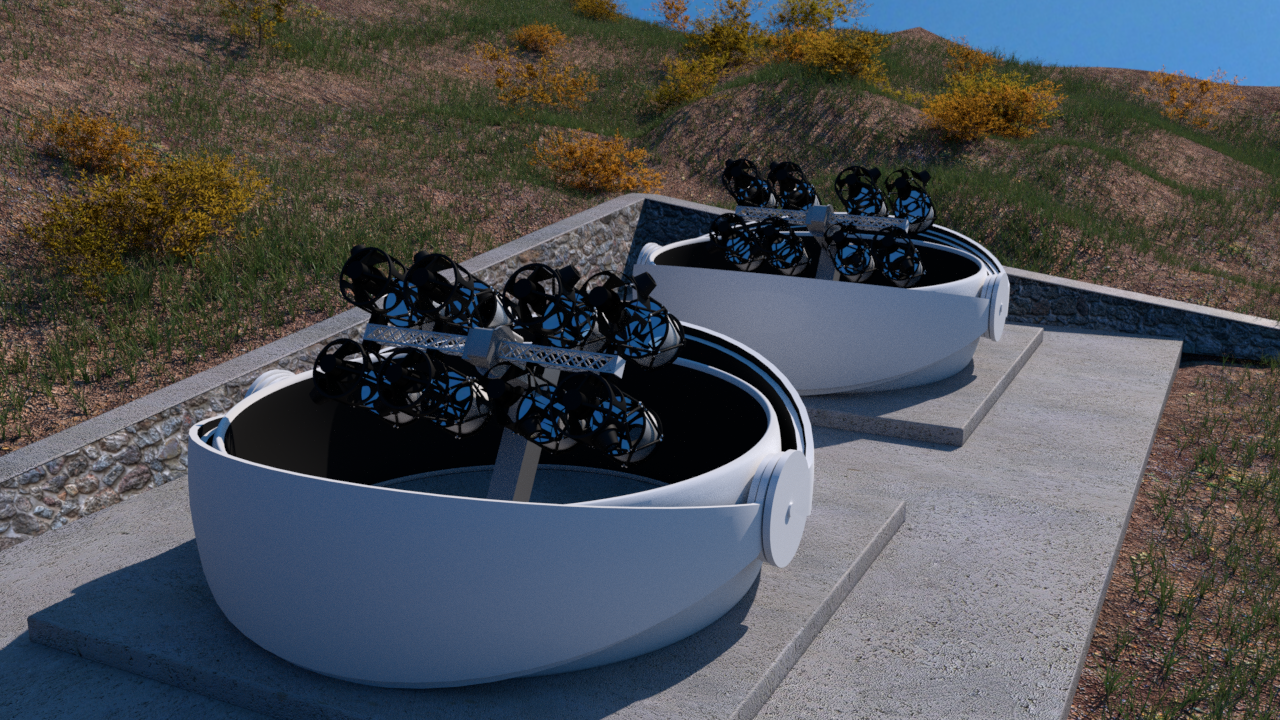
\includegraphics[width=0.9\linewidth]{images/goto_render.png}
    \end{center}
    \caption[A rendering of a complete GOTO node]{
        A rendering of a complete GOTO node with two independent mounts.
    }\label{fig:goto_render}
\end{figure}

\end{colsection}

% ~~~~~~~~~~~~~~~~~~~~

\subsection{Motivation}
\label{sec:goto_motivation}
\begin{colsection}

Even before the first detection of gravitational waves it was recognised that, due to the issues described in the previous section, the best chance of reliably detecting counterparts quickly was with a series of dedicated, robotic, wide-field telescopes. Most nights the telescopes would normally be carrying out an all-sky survey on a fixed grid, but when a gravitation wave alert was received they would quickly change to covering the skymap. As robotic telescopes they would be quicker to respond than human-operated telescopes, meaning follow-up observations could begin automatically just minutes after an alert was issued.

Rapidly covering large areas of the sky maximises the chance of finding any possible counterpart before it fades from view, however any such observations are going to be contaminated by a huge number of unrelated transient and variable objects (recall the hundreds of thousands of detections by ZTF when searching for the S190425z counterpart). Therefore the difficulty in finding any counterpart is not just covering the search area, but being able to distinguish the needle from the haystack of other astronomical detections. The best way to reduce the number of candidate detections is temporally: any objects with detections prior to the gravitational wave event time could not be associated with it. In order to do this the project needs an as-recent-as-possible image of the same patch of sky, which necessitates the telescope carrying out an all-sky survey with as low a cadence (the time between observing each point of the sky) as possible.

\end{colsection}

% ~~~~~~~~~~~~~~~~~~~~

\subsection{Hardware design}
\label{sec:goto_design}
\begin{colsection}

The GOTO telescopes have been designed to cover a large field of view to a reasonable depth (19--20 mag) while being able to rapidly slew between targets, all for a reasonable cost. The full design, as shown in \aref{fig:goto_photo}, uses an array of of \SI{40}{\cm} \glspl{ut} attached to a boom-arm on a single fast-slewing mount. Using multiple smaller instruments on one mount is a design already used by several survey and wide-field telescopes, such as the All-Sky Automated Survey for Supernovae \glsadd{asassn} \citep[ASAS-SN,][]{ASAS-SN} or Warwick's existing telescope on La Palma SuperWASP \glsadd{wasp} \citep{SuperWASP}. This modular design provides a cost-effective way of reaching the desired field of view, while also allowing the project to be scaled up as funding allows.

The prototype telescopes and mount were constructed by APM Telescopes\footnote{\url{https://www.professional-telescopes.com}}. Each UT is a fast Wynne-Newtonian astrograph with a focal ratio of f/2.5, and each uses off-the-shelf camera hardware from \glsfirst{fli}\footnote{\url{https://www.flicamera.com}}. The FLI MicroLine cameras each use a 50 megapixel sensor from ON Semiconductor\footnote{\url{https://www.onsemi.com}}, which gives each UT a field of view of approximately 6 square degrees with a pixel scale of \SI[per-mode=symbol]{1.2}{\arcsec\per\pixel}. A full GOTO telescope will have eight UTs per mount, giving an overall field of view of \SI{40}{\square\deg} (accounting for some overlap between cameras). A sample frame taken with one UT is shown in \aref{fig:fov}, which also gives a comparison of the GOTO field of view to other projects.

\begin{figure}[p]
    \begin{center}
        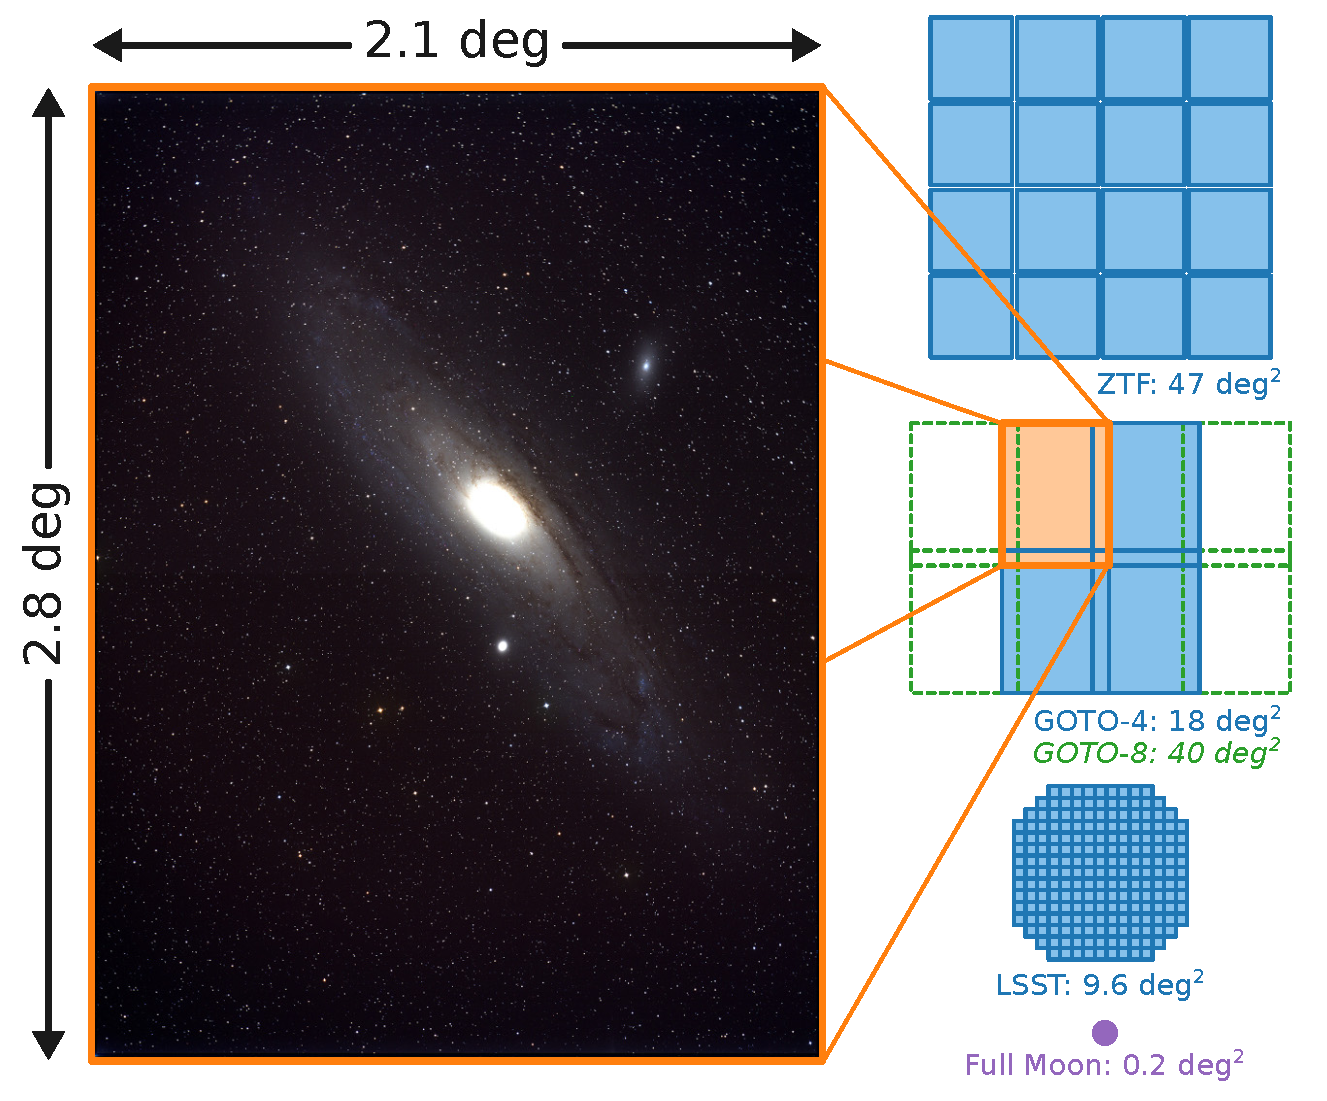
\includegraphics[width=\linewidth]{images/fov.pdf}
    \end{center}
    \caption[GOTO's field of view compared to other projects]{
        GOTO's field of view compared to other projects. On the left is a commissioning image of M31 taken with one of GOTO's cameras, showing the wide field of view of a single unit telescope. Four of these UTs form the initial 18 square degree survey tile, to be increased to 40 square degrees in the full 8-UT system. On the right the GOTO FoV is compared to two similar projects: the Zwicky Transient Facility \glsadd{ztf} \citep[ZTF,][]{ZTF} and the Large Synoptic Survey Telescope \glsadd{lsst} \citep[LSST,][]{LSST}.
    }\label{fig:fov}
\end{figure}

Each unit telescope is fitted with a filter wheel with several wide-band coloured filters, which can be used for additional source identification. The telescopes are housed in an Astrohaven clamshell dome\footnote{\url{https://www.astrohaven.com}}, which when fully open allows an unrestricted view of the sky. This means that the telescope does not need to waste time waiting for the dome to move before slewing to a new position, and can instead move from observing one portion of the sky to another as fast as possible.

Each GOTO site is anticipated to host two domes, as shown in \aref{fig:goto_render}, with a total of 16 unit telescopes giving an instantaneous field of view of approximately \SI{80}{\square\deg}. Having two independent mounts allows the sky to be surveyed at a higher cadence, and also gives more options for survey and transient follow-up strategies. For example, the two mounts could observe separately, each observing a different patch of the sky, in order to cover the skymap as fast as possible. Alternately they could combine to observe the same field to a greater depth. Another option is for each mount to observe using a different filter, to get immediate multicolour information on any detected sources.


\end{colsection}

% ~~~~~~~~~~~~~~~~~~~~

\subsection{Image processing and candidate detection}
\label{sec:gotophoto}
\begin{colsection}

\begin{figure}[t]
    \begin{center}
        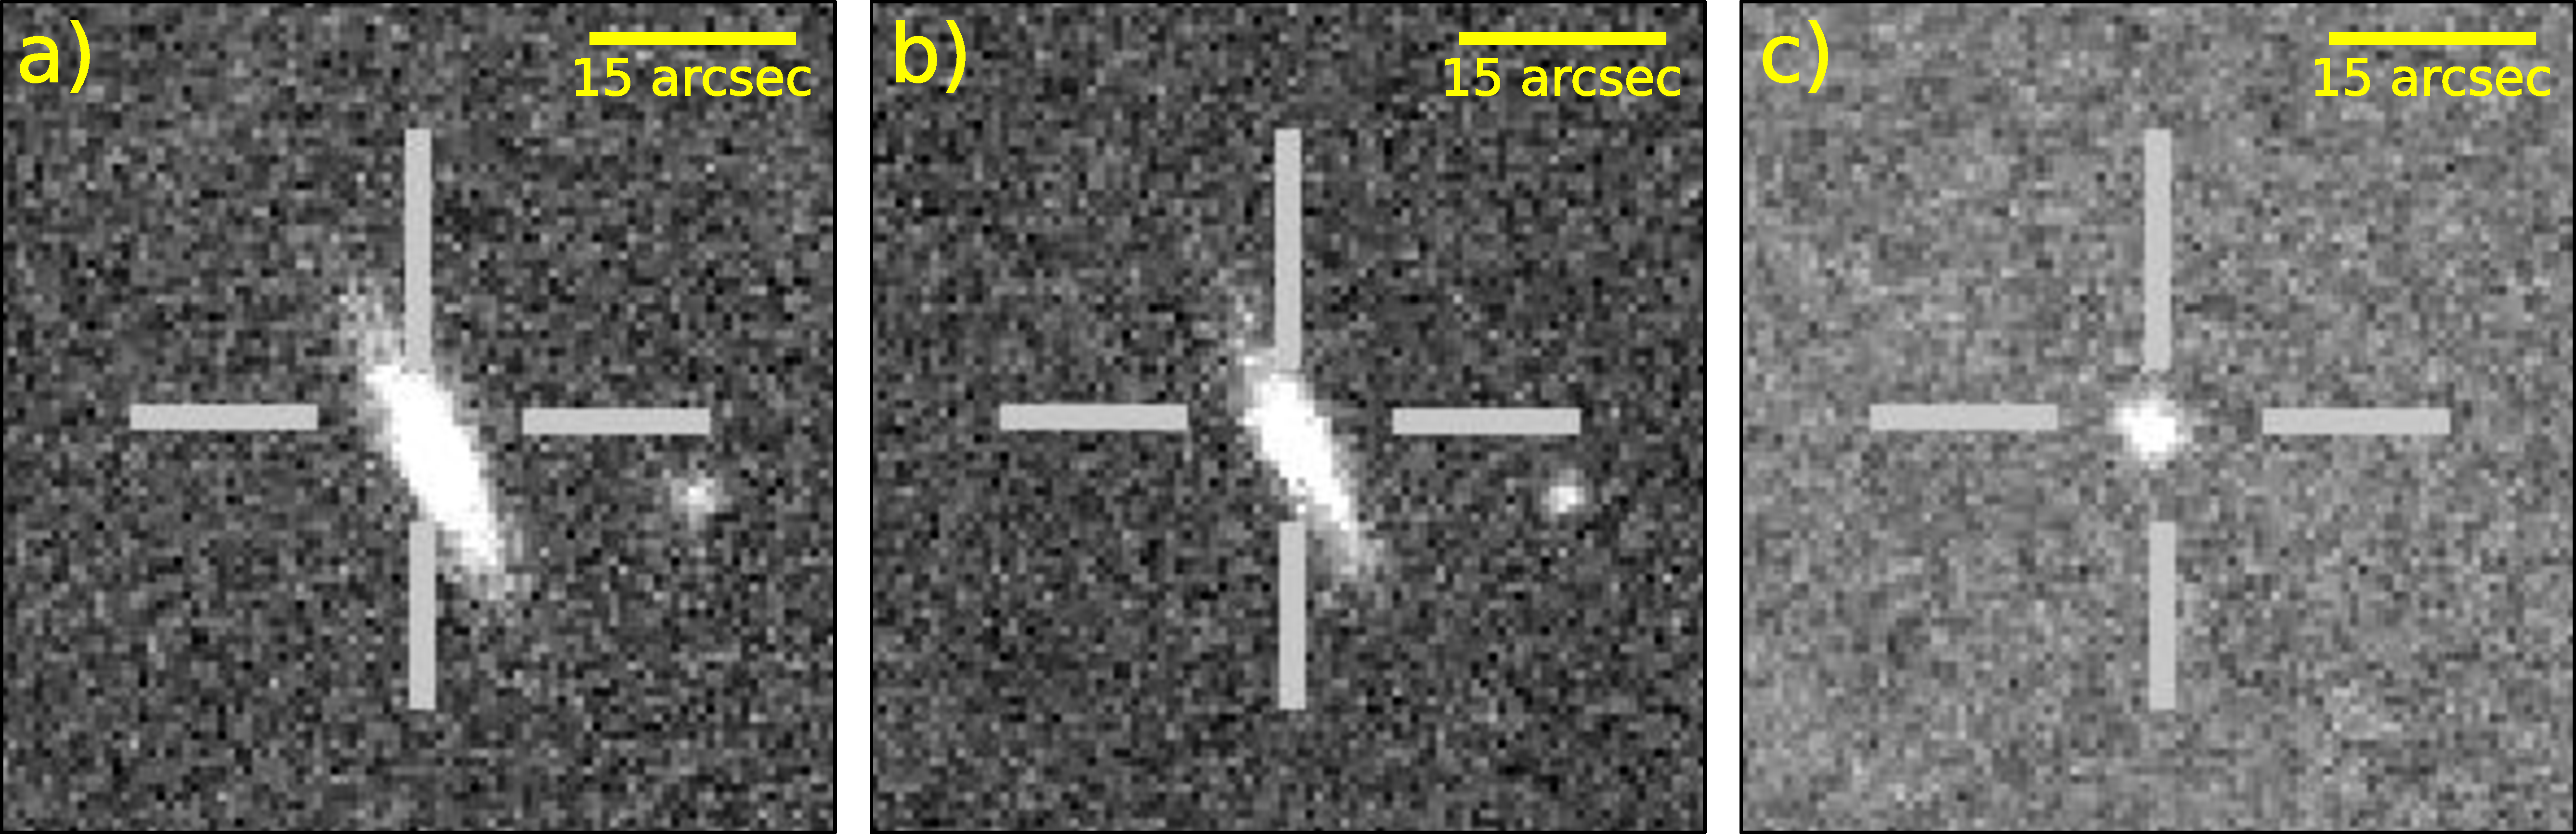
\includegraphics[width=\linewidth]{images/diffimg.pdf}
    \end{center}
    \caption[The detection of SN 2019bpc through difference imaging]{
        The detection of Type Ia supernova SN 2019bpc by the GOTOphoto difference imaging pipeline. The new exposure on the left (a) has the reference image (b) subtracted to give the difference image on the right (c), where the new source is clearly visible.
    }\label{fig:diffimg}
\end{figure}

The GOTO project requires handling a huge amount of data. Each output from the 50~Mpx cameras produces 100~MB image, GOTO typically takes three \SI{60}{\second} exposures per pointing and on average observes $\sim130$ targets each night. Just the prototype 4-UT system produces on the order of 150~GB every day, and a full multi-site GOTO system would produce close to 400~TB per year. In order for real-time transient detection each set of images needs to be processed in the approximately three minutes between each target, and due to the wide field of view each image will contain many thousands of sources. Processing the images is therefore not an easy task. In order to do this a real-time data flow system has been developed called GOTOflow, which is used to run the GOTO pipeline GOTOphoto.

GOTOphoto calibrates each image and combines each set of three, which increases the effective depth while also accounting for moving targets between the two exposures. New or changed sources are then detected using the method of difference imaging, as shown in \aref{fig:diffimg}. This requires a master reference image at each position in the sky, which is continuously built up from the all-sky survey. Any apparently new sources are then added to a detection database, and are also checked against historic observations to discount any sources which had been observed previously (for example, variable stars on the edge of the detection depth might fade in and out of visibility). Candidate sources are also checked against existing source catalogue, as well as against lists of known minor planets and other transients.

New candidates are then currently presented for human vetting, through a web interface called the GOTO Marshal. Collaboration members can check each candidates and flag them either as potential astrophysical sources or junk detections. Work is ongoing across the collaboration on machine-learning projects for transient detection and identification, which would use the human responses from the Marshal to attempt to automatically classify the most probable candidates.

\end{colsection}

% ~~~~~~~~~~~~~~~~~~~~

\subsection{Deployment and future expansion}
\label{sec:goto_expansion}
\begin{colsection}

The 4-UT GOTO prototype shown in \aref{fig:goto_photo} was inaugurated in the summer of 2017. The telescope is located at the \glsfirst{orm_lapalma} on La Palma in the Canary Islands, at the site shown in \aref{fig:orm}. After some hardware issues the telescope is now fully operational: since February 2019 GOTO has been carrying out a continual all-sky survey, and as of the start of the third LIGO-Virgo observing run (O3) in April 2019 it has been actively following-up gravitational wave events when they occur.

The next stage in the GOTO project will be the addition of the second set of four unit telescopes to the existing mount, due in late 2019. Following that funding for a second mount and initial set of unit telescopes has already been secured, and a second dome has already been constructed on La Palma. The second mount is therefore expected to be commissioned in the next few years.

La Palma is one of the best observing site in the northern hemisphere, and and was already home to several telescopes operated by GOTO collaboration members. It was therefore an obvious choice for the location of the first GOTO node. Ultimately a second, complimentary node is planned to be built in the southern hemisphere, most likely in Australia. Having a site in both hemispheres allows the entire sky to be visible, and as Australia is on the opposite side of the Earth from La Palma the two sites would provide almost 24-hour observing coverage. This second node would also host two GOTO telescopes with 8 UTs each, and the two sites combined would be able to survey the entire visible sky every 1--2 days. As GOTO grows it is anticipated that the telescopes at both sites will be operated as a single observatory, meaning observation scheduling will be optimised between each site and the output data will be unified into a single detection database.

\begin{figure}[p]
    \begin{center}
        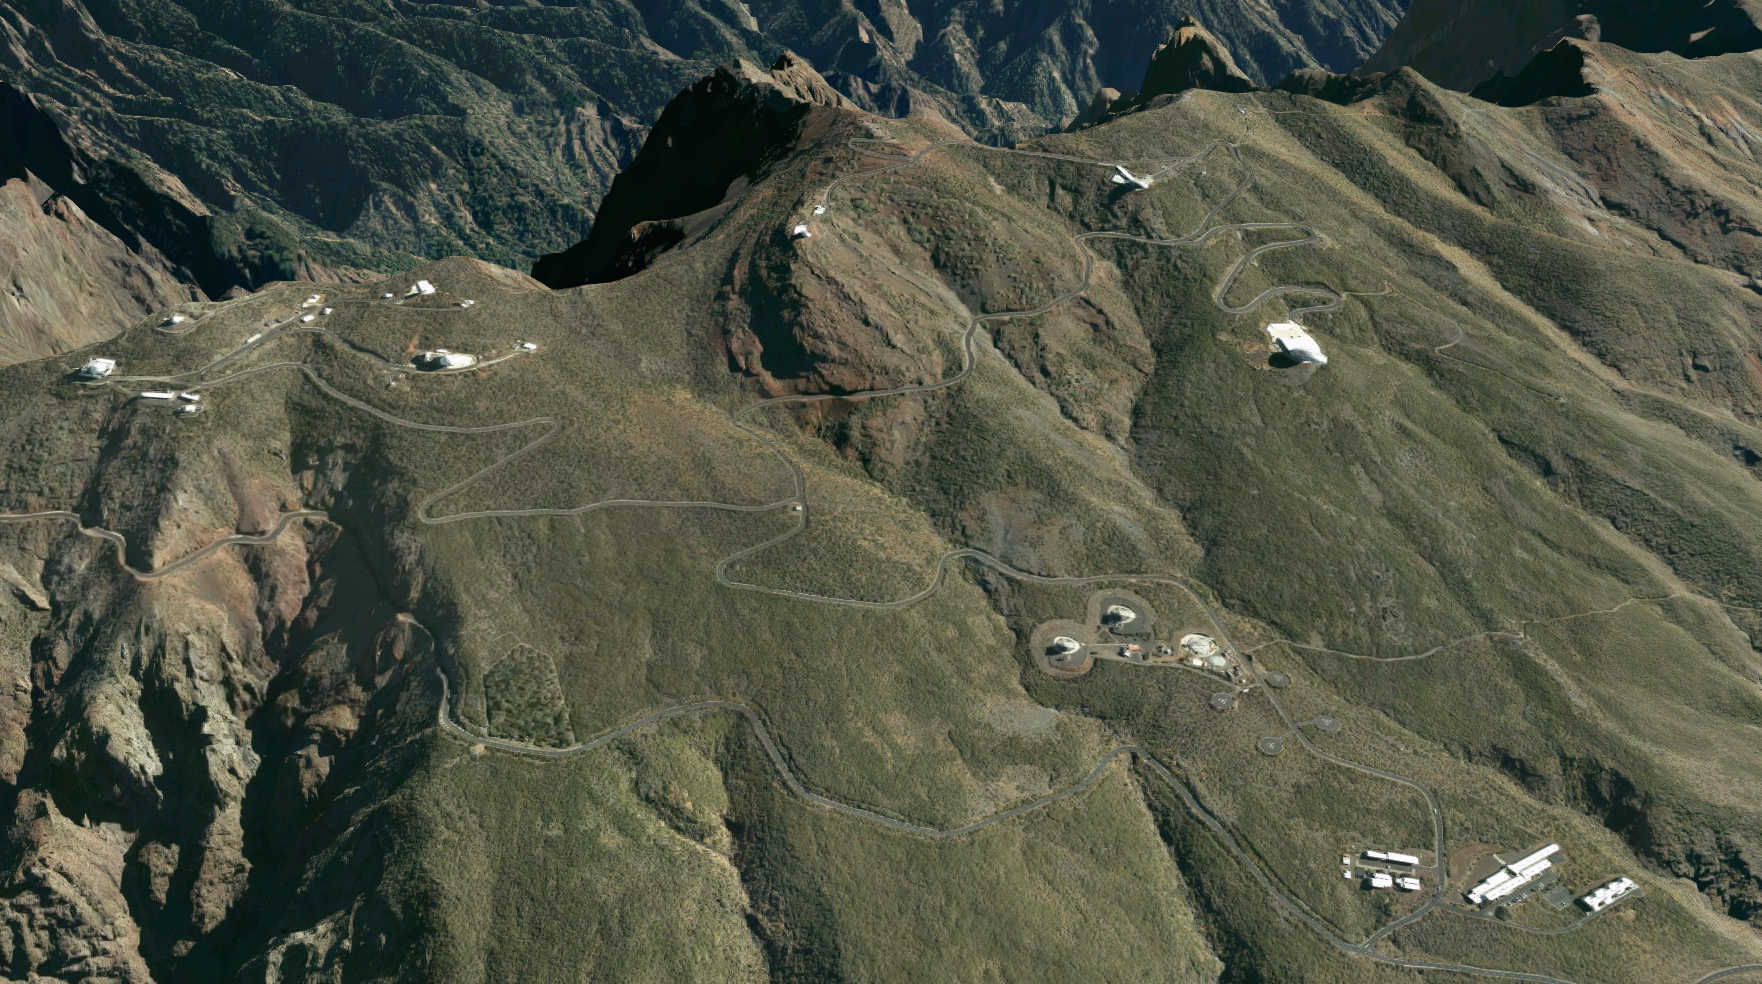
\includegraphics[width=\linewidth]{images/orm.pdf}
    \end{center}
    \caption[The location of GOTO and other telescopes on La Palma]{
        The location of GOTO and other telescopes at the Observatorio del Roque de los Muchachos on La Palma, including the sites of proposed and under-construction projects in \textcolorbf{Goldenrod}{yellow}. GOTO, marked in \textcolorbf{BlueGreen}{blue}, is located on the east side of the observatory, close to the edge of the caldera. The lower image shows the eastern part of the ORM and the telescopes surrounding GOTO, including the other Warwick-operated telescopes (W1m and SuperWASP) and the Sheffield/Durham-operated pt5m (on the roof of the WHT building) in \textcolorbf{ForestGreen}{green}. Satellite images taken from Google Maps.
    }\label{fig:orm}
\end{figure}

\clearpage

\end{colsection}

% ~~~~~~~~~~~~~~~~~~~~

\end{colsection}

% ########################################

\newpage
\section{Thesis outline}
\label{sec:outline}
\begin{colsection}

This thesis details my work on the GOTO project carried out between 2015 and 2019.

My primary role within the collaboration was to develop the software needed for GOTO to operate as an autonomous telescope. On the basic level, the hardware design of GOTO --- with multiple unit telescopes attached to each mount --- required custom software which could operate all the cameras in sync. Each unit telescope is also equipped with a filter wheel and a focuser, which would also need to be controlled in parallel. Additional control software was also required to move the mount, open and close the dome, and control any other pieces of on-site hardware.

The next stage of the control system development was writing the software that would operate the telescope without human involvement. The routine nightly operations (move to a target, take an exposure, repeat until sunrise) would need to be supported, and in addition standard observational tasks such as taking calibration frames and focusing the telescopes needed to be automated. Crucially the control system required robust and reliable systems for monitoring the weather and the hardware status, and in the case of an emergency it had to be able to close the dome or recover from any problems without immediate human intervention.

In order for a telescope to observe autonomously it needs to be able to know what targets to observe and when. Therefore GOTO needed an automatic scheduling system, which had to be able to handle two distinct operational modes:\@ carrying out the all-sky survey for the majority of the time, but quickly switching to follow-up any gravitational wave alerts (or other transient events) when triggered. For the all-sky survey a series of tiled pointings had to be to be defined and alert observations should be mapped onto the same grid, to enable the pipeline to carry out difference imaging. Reacting quickly to any alerts is vital, so GOTO needed a robust alert monitoring system that could determine the optimal follow-up strategy for each event.

Finally, as described in \aref{sec:goto_expansion}, GOTO is envisioned as a modular project with an increasing number of telescopes and sites, eventually operating as a multi-site observatory. This future expansion had to be taken into account in the design of both the hardware control and scheduling systems.

This thesis is arranged as follows:
%
\begin{itemize}
    \item In \nref{chap:hardware} I describe my work characterising the GOTO hardware and optical systems prior to its deployment.
    \item In \nref{chap:gtecs} I introduce the software I developed to control the GOTO hardware.
    \item In \nref{chap:autonomous} I describe the additional autonomous level of software I wrote to allow GOTO to operate as a robotic telescope.
    \item In \nref{chap:scheduling} I examine in detail the functions used to prioritise and schedule GOTO observations.
    \item In \nref{chap:tiling} I describe how GOTO observations are mapped onto an all-sky grid, and how it is used to observe gravitational-wave skymaps.
    \item In \nref{chap:alerts} I describe the software systems used to receive and process astronomical alerts, including gravitational wave detections.
    \item In \nref{chap:commissioning} I detail my work during the deployment of the GOTO prototype and subsequent development of the on-site system.
    \item In \nref{chap:multiscope} I examine the future expansion plans of GOTO, and detail simulations I carried out to quantify the benefits of multiple telescopes and sites.
    \item Finally, in \nref{chap:conclusion} I present concluding remarks and some suggestions for future project development.
\end{itemize}

\end{colsection}

% ########################################
